\documentclass[12pt]{article}
\usepackage{amssymb}
\usepackage{amsmath}
\usepackage{esdiff}
\usepackage[margin=1in]{geometry}
\usepackage{enumitem}
\usepackage{graphicx}
\usepackage{fancyhdr}
\usepackage{caption}
\usepackage{sidecap}
\usepackage{float}
\pagestyle{fancy}
\setlength\parindent{0pt}
\usepackage{mathtools}
\graphicspath{ {images/} }

\setlength{\headheight}{15 pt}
\lhead{Andrew Fischer}
\chead{HW 09 - Project Proposal}
\rhead{CIS 120}

\begin{document}
  
  \section*{CIS 120 Game Project Proposal}
  \begin{center}  
    \begin{tabular}{cc}
      \vspace{-.25cm} 
      \texttt{aff}                 & Max McCarthy   \\
      \makebox[2.5in]{\hrulefill}  &     \makebox[2.5in]{\hrulefill} \\
      PennKey                      &     TA consulted with \\
    \end{tabular}
  \end{center}
  
  
  \subsection*{General Questions}
  
  \textbf{What game are you planning to implement? If it is a game of your own 
  design, or not especially well-known, provide a 2-3 sentence description of
  the game.
  }

  I plan to create an role playing game (RPG) inspired by some of my favorite 
  classic games, such as \textit{Earthbound} and \textit{Fallout}. The game will
  include motion on a grid, enemy encounters, and a leveling/status system.
  \bigskip
  
  \textbf{What classes and interfaces do you plan to create? How will the 
  different components of your game (the model, the GUI, etc.) interact?
  }

  The most complex interface will most likely be the \texttt{Character}
  interface. THis inteface will have subclasses for the player character as well
  as NPCs. The NPC classes will be inhereted by friendly (non-attacking) and
  non-friendly characters.

  In addition, it is possible I will need a \texttt{Tile} interface for
  ground tiles. Tiles can be walkable and non-walkable, can be on different planes, can
  cause actions to take place (i.e.stairs to another floor), and could possibly
  have hazards (i.e., spikes, lava, etc.). Using a class heirarchy could be
  necessary if a more simple data structure will not suffice.
  \bigskip

  \textbf{What do you think will be the most challenging thing to implement?
  }
  I think the walking grid will be most complicated to implement, as there are
  so many variations on state that can occur. I will need to check for a number
  of things and make sure that I am using a suitible data structure to hold
  information about the ground state.

  \subsection*{Core Concepts}

  \begin{enumerate}[leftmargin=\labelsep]
    \item Concept 1: \textbf{2D Array}
    
    \textbf{What specific feature of your game will be implemented using this
      concept?
   }
   
    A 2D array of some sort will be used to represent the layout of the current 
    room the player is in. It could be as simple as a 2D array holding certian 
    values depending on the type of tile at that coordinate (i.e., 0 for empty, 
    1 for non-walkable, 2 for walkable, etc.), or, it could hold an array of 
    \texttt{Tile} elements each with their own unique qualities.
    
    \textbf{Why does it make sense to implement this feature with this concept?
      Justify why this is a non-trivial application of the concept in question.
    }
    
    The 2D array is appropriate as it is a good model for holding data of this 
    type and is flexible enough to allow me to store whatever data I deem 
    necessary in it. In addition, it would allow extensibility if needed.
    
    \begin{SCfigure}
      \centering
      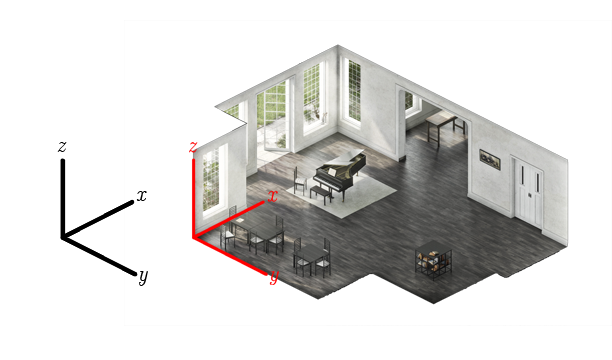
\includegraphics[width=3in]{iso}
      \captionsetup{labelformat=empty}
      \caption{
        \textit{Stretch Goal: Isometric Grid.}
        An isometric grid translates a 2D grid into a pseudo 3D space where all 
        dimentions are reprented equally. I find it to be an incredibly 
        interesting concept and hope to attempt to implement it if I have enough
        time. Due to the flexible implementation outlined above, I don't believe
        this will be too hard.
      }
    \end{SCfigure}
    
    \bigskip
    
    \item Concept 2: \textbf{Inheretence \& Subtyping}
    
    \textbf{What specific feature of your game will be implemented using this
     concept?}
    
    An inheritance heirarchy will be used to model the different characters in 
    the game, including both the player character and NPCs. In addition, 
    Inheretence may be used for the floor tiles.
    
    
    \textbf{Why does it make sense to implement this feature with this concept?
     Justify why this is a non-trivial application of the concept in question.}


    There are many different types of characters, but all will share some 
    qualities, including health, an invintory, a name, etc. Having a character 
    interface will ensure consistency in implementation while allowing each type
    of character to have unique qualities and rules.

    \item Concept 3: \textbf{Novel Recursive Data Structure} 
    
    \textbf{What specific feature of your game will be implemented using this
     concept?}
    
    \item 
    I hope to incorporate \"roguelike\" elements into the game, such as random 
    room generation. Using a unqiue recursive algorithm, I hope to create and
    interesting and new experience every time the game is loaded. 
    

    \textbf{Why does it make sense to implement this feature with this concept?
      Justify why this is a non-trivial application of the concept in question.
    }


    Using an interesting and unique recursive structure to generate levels would
    not only prove to be a fun coding challenge but would make each time the
    game is played a unique experience. Every level would be different and
    (hopefully) fun.

    \item Concept 4: \textbf{Testable Components}
    
    
    \textbf{What specific feature of your game will be implemented using this concept?
    }
    
    
    If some type of algorithm will be generating rooms, we will need to make
    sure that that algorithm is never failing (i.e., creating unplayable or
    impossible levels.) Using \texttt{JUnit} testing to ensure the level
    generator is working as expected will be important and make testing
    easier.


    \textbf{Why does it make sense to implement this feature with this concept?
      Justify why this is a non-trivial application of the concept in question.
    }


    The level generator will be some type of mathmatical equation to create an
    array of floor tiles. The tiles must be traversable and rooms will be
    required to have certain qualities. Using \texttt{JUnit} tests seems
    logicsal to make sure each component is working as expected.
    
  \end{enumerate}

\end{document}